\subsubsection*{$\Sigma \Delta$ modulator.}
 We illustrate the interest of timed pattern generation with a $\Sigma \Delta$ modulator which is an important component of $\Sigma \Delta$ analog-to-digital converters. Such converters have been widely used for analog signals of a large range of frequencies. Practical quantizers have a limited input and output ranges, which may lead them to saturation. We apply our methods of signal generation to test if a saturation can occur in a $\Sigma \Delta$ modulator. We use a behavioral model of a second-order modulator specified using Simulink\textsuperscript{\textregistered}, which takes into account most non-idealities \cite{Brigati99}, including sampling jitter, integrator noise, op-amp parameters (finite gain, finite bandwidth, slew-rate and saturation voltages). In terms of model complexity, this Simulink model is heterogeneous including embedded Matlab code and mixing discrete-time and continuous-time components, which goes beyond the applicability of the existing formal verification tools. Simplified discrete-time $\Sigma \Delta$ modulator model without non-idealities, for which it is possible to derive its dynamics equations and thus optimization can be formulated and solved using optimization \cite{DangDM04} and statistical model-checking \cite{ClarkeDL10}.
\begin{figure}[htbp]
\resizebox{0.85\textwidth}{!}{
\begin{tikzpicture}[->,>=stealth',shorten >=1pt,auto,node distance=2.1cm, initial text={}]
   \node [accepting,state] (q0)                      {$q_4$};
   \node[accepting,state]          (q1) [right of=q0,yshift=-0.8cm]         {$q_5$};
   \node[accepting,state]          (q2) [left of=q1,yshift=-0.8cm]         {$q_6$};
   \node[accepting,state]          (q3) [left of=q0,yshift=-0.8cm]         {$q_3$};
   \node [accepting,state] (q2bis)    [left of=q3]                  {$q_2$};   
   \node [accepting,state] (q1bis)    [left of=q2bis]                  {$q_1$};
   \node [initial,accepting,state] (q0bis) [left of=q1bis]                      {$q_0$};
   \path (q0) edge [bend left] 
   node {$\begin{array}{c}
         x_1\in (1,6)\\ x_1:=0
   \end{array}$} (q1);
   \path (q1) edge [bend left] 
   node {$\begin{array}{c}
         x_2\in (1,6)\\
        x_2:=0
   \end{array}$} (q2);
   \path (q2) edge [bend left] 
   node {$\begin{array}{c}
         x_3\in (1,6)\\ x_3:=0
   \end{array}$} (q3);
   \path (q3) edge [bend left]  
   node {$\begin{array}{c}
         x_4\in (1,6)\\
        x_4:=0
   \end{array}$} (q0);
   \path (q0bis) edge node [above] {$\begin{array}{c}x_1\in (0,6)\\ x_1:=0\end{array}$} (q1bis);
   \path (q1bis) edge node [above] {$\begin{array}{c}x_2\in (0,6)\\ x_2:=0\end{array}$} (q2bis);
   \path (q2bis) edge node [above] {$\begin{array}{c}x_3\in (0,6)\\ x_3:=0\end{array}$} (q3);
\end{tikzpicture}
}
%\begin{tikzpicture}[->,>=stealth',shorten >=1pt,auto,node distance=1.2cm, initial text={$c=0$}]
%   \node [initial,state,accepting] (q0)                      {$0$};
%      \path (q0) edge [loop above]  node [above]  {$\begin{array}{c} c'=2 c+\lfloor t \rfloor,
%      c'_0=\lfloor t \rfloor,\\ c'_{-1}=c_0, c'_{-2}=c_{-1}, c'_{-3}=c_{-2},\\
%      \textcolor{purple}{c_0+c_{-1}+c_{-2}+c_{-3} \in\{1,2\}}\end{array}$} (q0);
%\end{tikzpicture}
\caption{A timed automaton for the period constraint.}
 \label{fig:4.5clocks}
\end{figure}
%(see Fig.~\ref{fig:DeltaSigma}),
%\begin{figure}[!ht]
%  \centering
%  \includegraphics[width=0.9\textwidth]{figures/DSfig.pdf}
%  \caption{$\Sigma \Delta$ model with non-idealities \cite{Brigati99}.\label{fig:DeltaSigma}}
%\end{figure}%\vspace{-1cm}
~\\
The timed automaton in Figure \ref{fig:4.5clocks} specifies a class of quasi-periodic signals with uncertain period drifting duration that ranges between $1$ and $6$. The period duration can be scaled to consider the frequency range of interest. We discretise the signal value space and associate each transition label with a signal value range. The first transitions are used to model uncertainty in phase shift. The transitions should reflect some bounded variability condition. Then the signals are constructed by linear interpolation between the values of the time instants. The absence of saturation can be expressed as a simple STL property, which states that throughout the simulation duration, the absolute value of the output of the saturation block in the first integrator is always smaller than the saturation voltage value (which is $1.145$). We generate a set of $50$ timed words using uniform sampling \cite{BBBK16}. Indeed the automaton n Figure \ref{fig:4.5clocks} is compact and thus used for illustration; for pattern generation we use an automaton with more locations for more refined value intervals, and the signal period varies from $10$ to $16$. The scaling factor for the period is $6 \times 10^{-7}$. For the optimization part, we use Algorithm \ref{algoSolverCombination} for guided  combination of metaheuristics, with $30$ time instant parameters. This experiment allows observing that combining optimization with timed pattern generation allows us to falsify the absence of saturation after using $22$ generated timed patterns. For comparison purposes, we designed a custom strategy to encode the timed automata constraint: we created a domain with variable time instants, and for each signal generated, we compute the period drifting and check whether it lies in the given bounds. Over $100$ signals generated this way, we reject $37$ (see Figure~\ref{fig:reject}). We note that this type of encoding was doable for this example, but can be much more involved for more complex TA and lead to much higher rejection rate, rendering falsification without our approach infeasible. 
\begin{figure}[htbp]
  \centering
  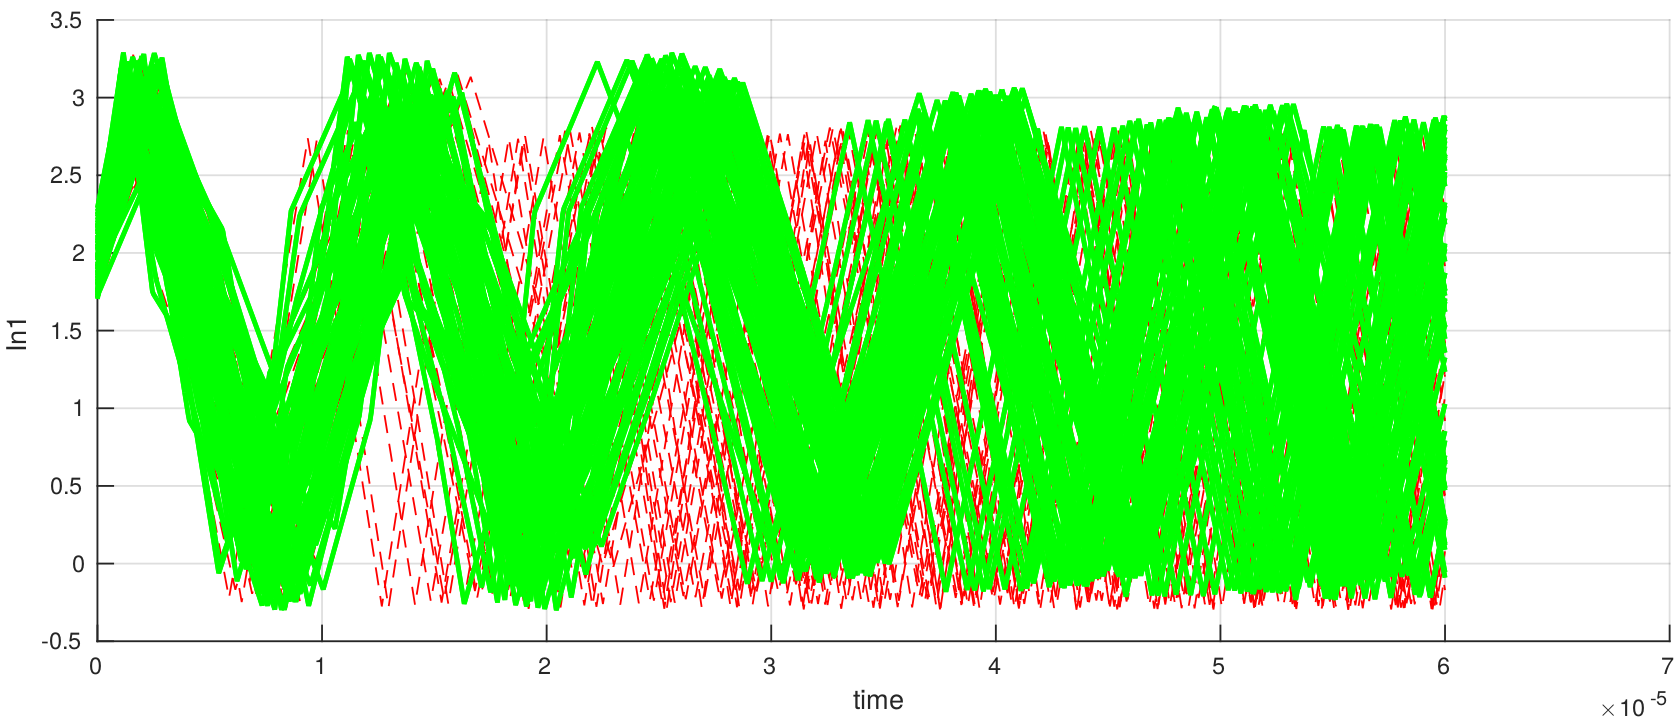
\includegraphics[width=\textwidth]{inputs_reject.png}
  \caption{The figure presents a set of $100$ signals generated with a custom method, of which 63 (green solid) satisfy the constraints of the timed automaton, and $37$ (red, dashed) do not.}
  \label{fig:reject}
 % \vspace{-3mm}
\end{figure}

